\documentclass[12pt]{article}
\usepackage[utf8]{inputenc}
\usepackage{hyperref}
\usepackage{geometry}
\usepackage{graphicx}
\usepackage{xurl}
\geometry{a4paper, margin=1in}

\title{Jawaban Tugas: Modifikasi Navbar Tailwind CSS}
\author{Aditya Dwi Nugroho (25.01.5252)}
\date{\today}

\begin{document}

\maketitle

\section{Tautan GitHub}
\url{https://github.com/AdityaDwiNugroho/Tugas_Tailwind_AMIKOM/blob/main/index.html}

\section{Tangkapan Layar Hasil Implementasi}

\subsection{Tampilan Desktop (Kondisi Default)}
\begin{figure}[h!]
    \centering
    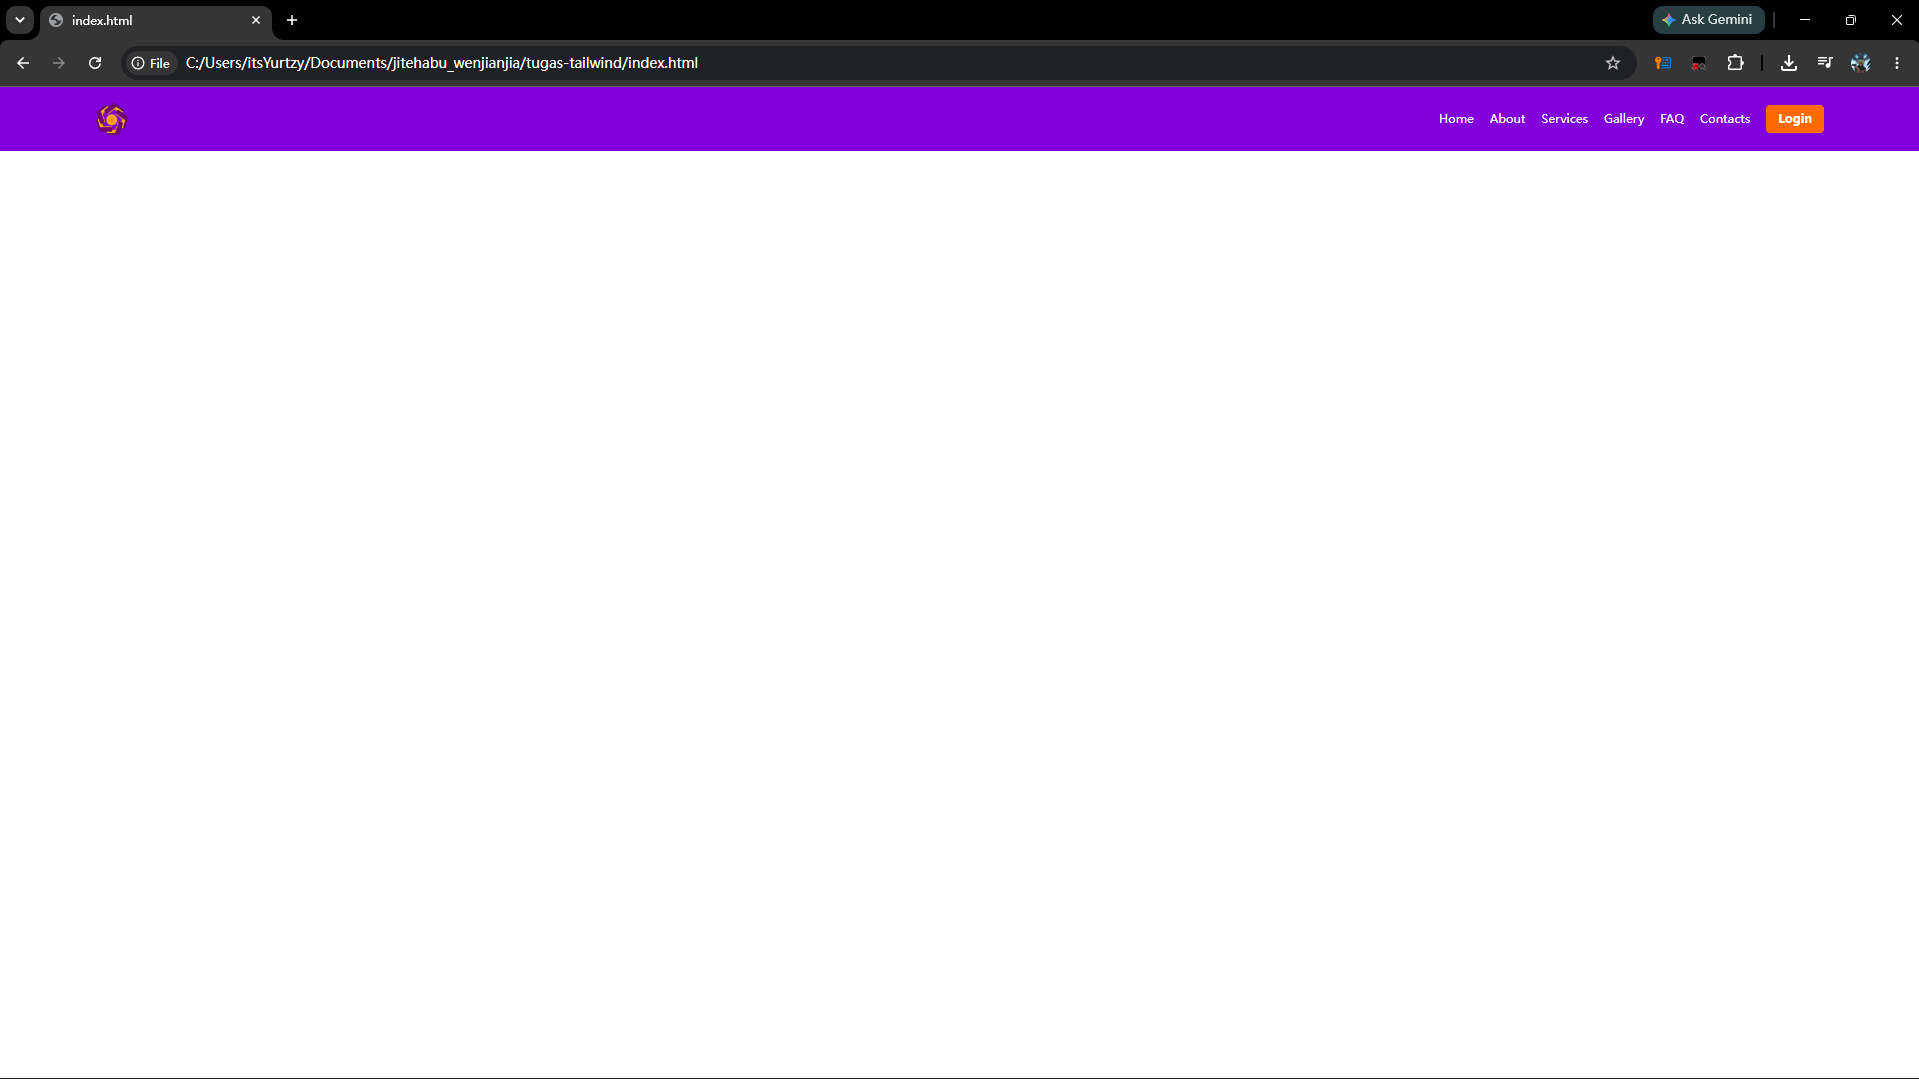
\includegraphics[width=0.9\textwidth]{desktop_default.png}
    \caption{Tampilan Desktop Default}
    \label{fig:desktop_default}
\end{figure}

\subsection{Tampilan Desktop (Hover Scaling Logo)}
\begin{figure}[h!]
    \centering
    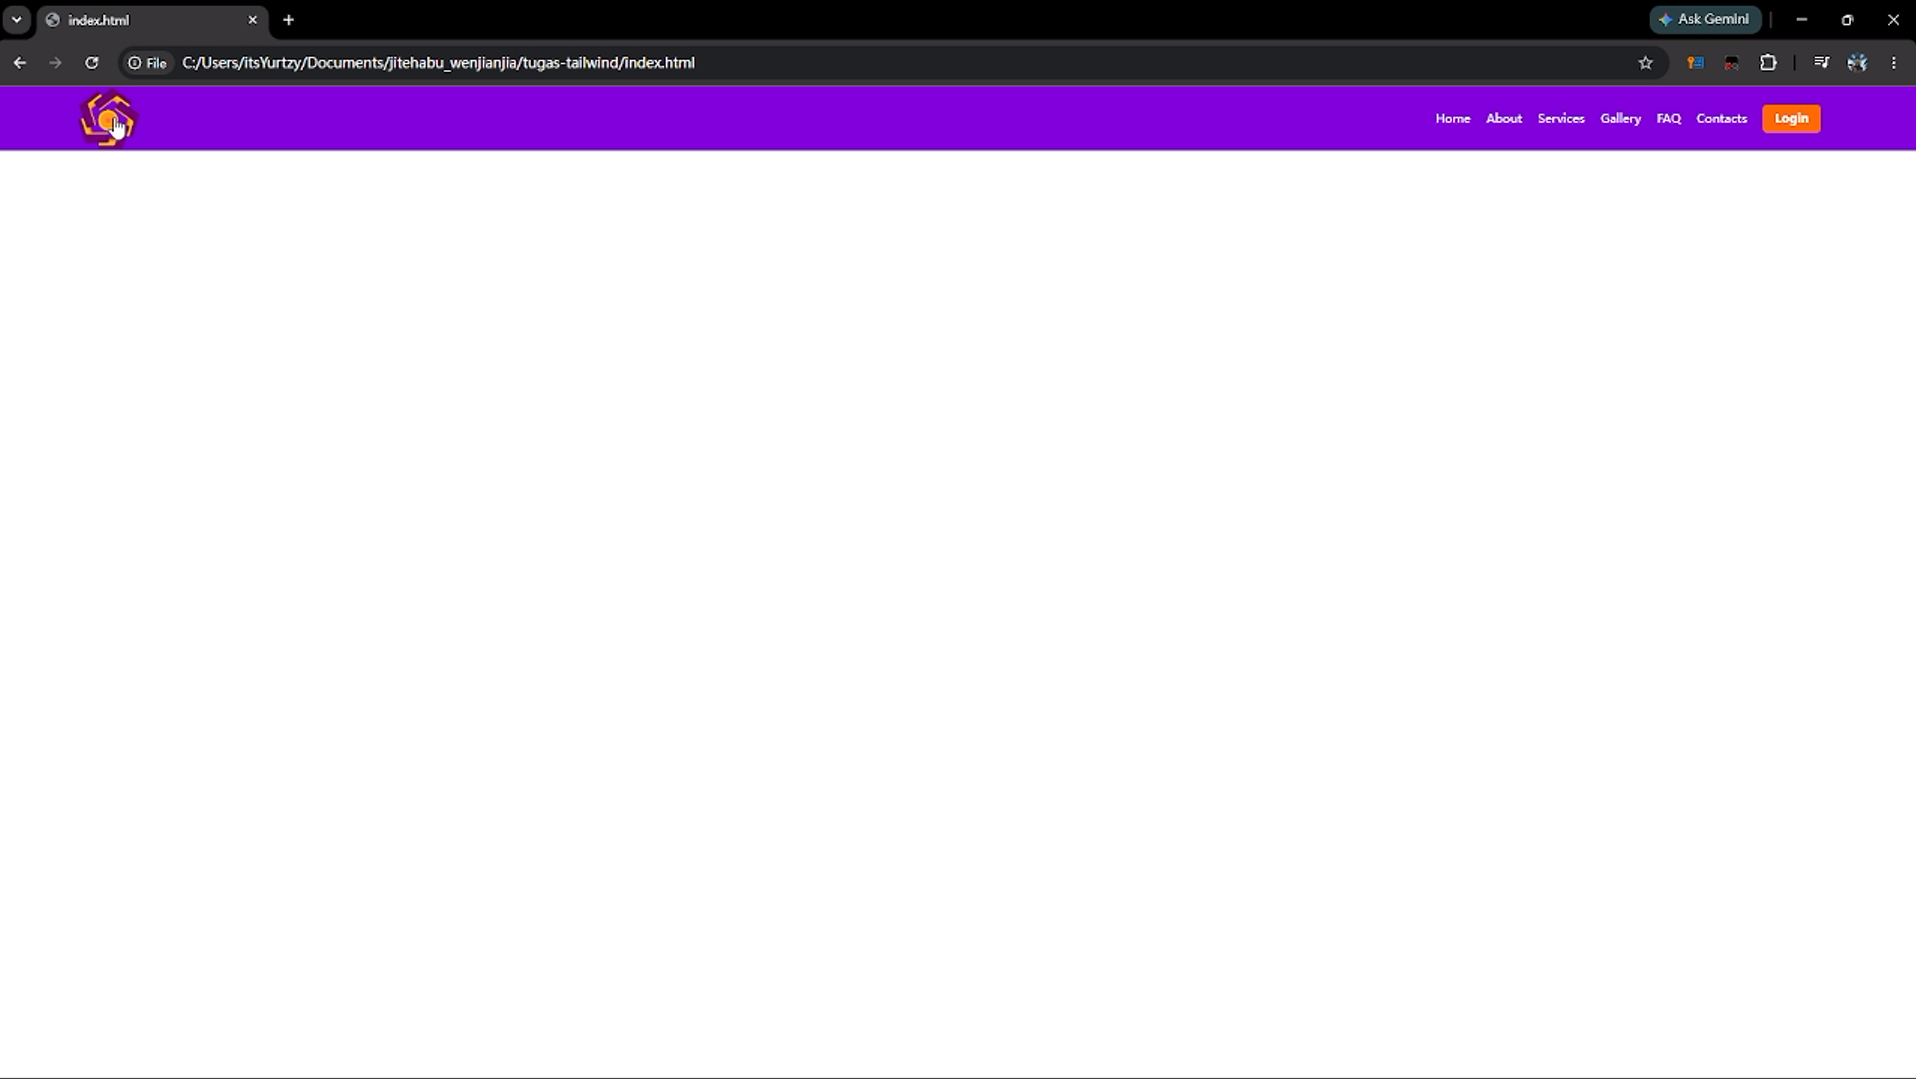
\includegraphics[width=0.9\textwidth]{logo_hover.png}
    \caption{Efek Hover Scaling Logo}
    \label{fig:logo_hover}
\end{figure}

\newpage

\subsection{Tampilan Desktop (Hover Link Menu)}
\begin{figure}[h!]
    \centering
    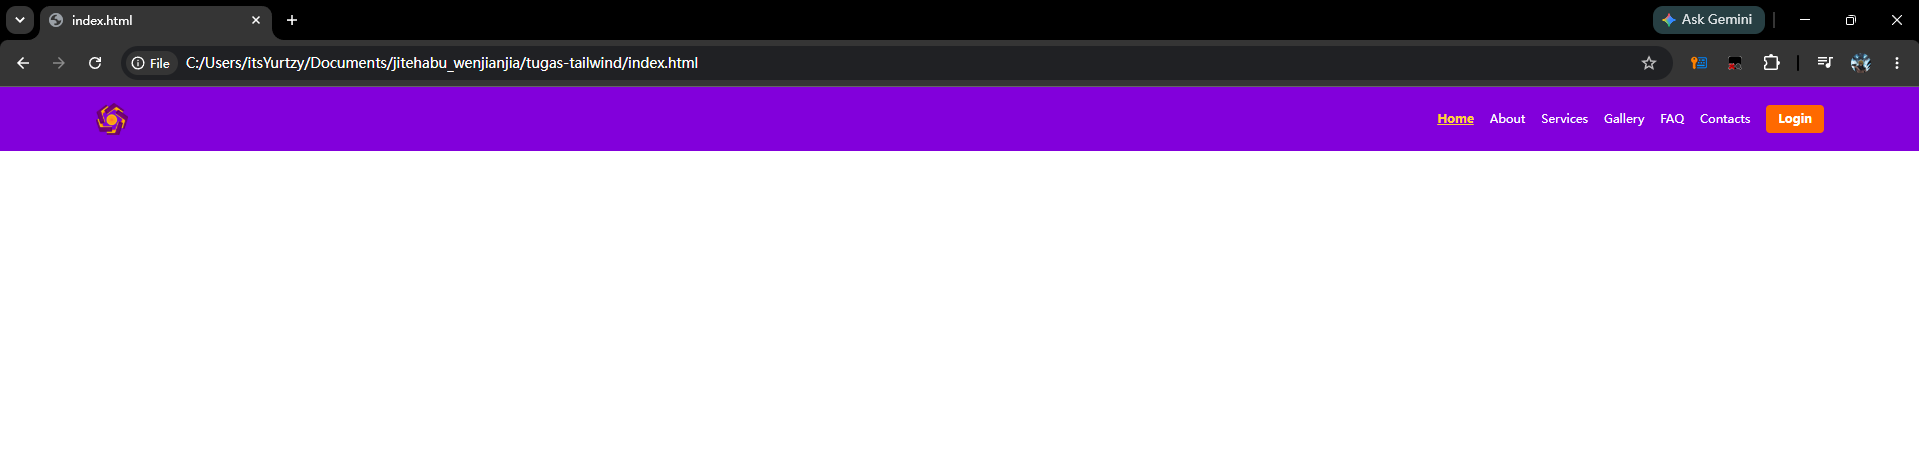
\includegraphics[width=0.9\textwidth]{link_hover.png}
    \caption{Efek Hover pada Link Menu}
    \label{fig:link_hover}
\end{figure}

\subsection{Tampilan Tablet (Surface Pro 7)}
\begin{figure}[h!]
    \centering
    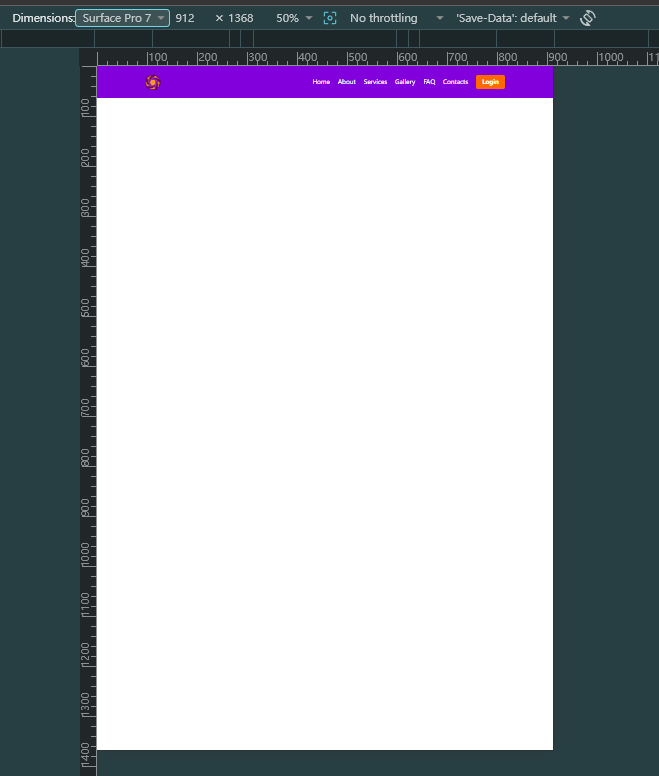
\includegraphics[width=0.75\textwidth]{tablet_surface.png}
    \caption{Tampilan Responsif pada Layar Tablet}
    \label{fig:tablet_surface}
\end{figure}

\newpage

\subsection{Tampilan Mobile (Samsung Galaxy S8+)}
\begin{figure}[h!]
    \centering
    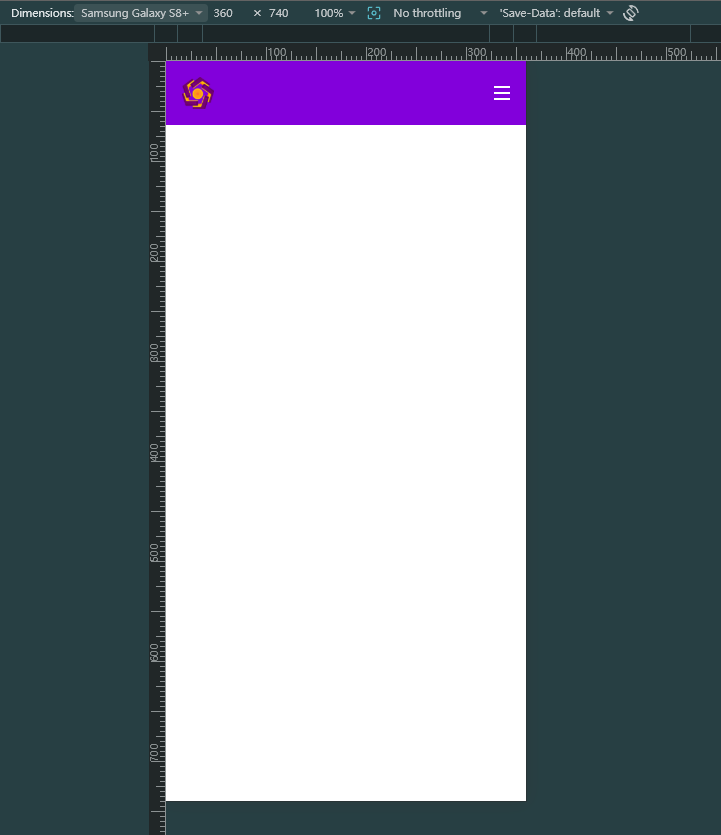
\includegraphics[width=0.45\textwidth]{mobile_galaxy.png}
    \caption{Tampilan Responsif pada Layar Mobile}
    \label{fig:mobile_galaxy}
\end{figure}

\newpage

\section{Penjelasan 10 Class Tailwind CSS}
Berikut adalah penjelasan 10 class Tailwind CSS yang digunakan pada navbar:

\begin{enumerate}
    \item \texttt{bg-purple-800}: Mengatur warna latar belakang (background) navbar menjadi ungu (shade 800).
    \item \texttt{flex}: Mengaktifkan model tata letak Flexbox untuk menyusun elemen secara horizontal atau vertikal.
    \item \texttt{justify-between}: Mendistribusikan elemen secara merata sehingga elemen pertama berada di kiri dan elemen terakhir di kanan.
    \item \texttt{items-center}: Meratakan elemen anak secara vertikal tepat di tengah-tengah flex container.
    \item \texttt{transition-transform}: Mengaktifkan efek transisi animasi khusus pada properti \texttt{transform} (seperti skala).
    \item \texttt{duration-300}: Menentukan durasi efek transisi selama 300 milidetik (0.3 detik).
    \item \texttt{hover:scale-110}: Membesarkan ukuran skala logo sebesar 110\% saat disentuh kursor (efek hover).
    \item \texttt{hidden}: Menyembunyikan elemen dari tampilan layar (\texttt{display: none}).
    \item \texttt{sm:flex}: Menampilkan elemen sebagai flexbox hanya pada layar ukuran sedang ke atas (breakpoint \texttt{sm}).
    \item \texttt{rounded}: Memberikan sudut membulat (\texttt{border-radius}) standar pada tombol Login.
    \item \texttt{bg-orange-500}: Memberikan warna latar belakang oranye pada tombol Login.
    \item \texttt{hover:bg-orange-600}: Mengubah warna latar belakang tombol menjadi oranye yang lebih gelap saat di-hover.
\end{enumerate}

\end{document}
